\section{Safety-Constrained CoC와 평가 방법}
\label{sec:method}

본 장의 목적은 모델이 실행 가드를 실제로 읽고 궤적 선택에 사용하는지 확인하는 방법을 설명하는 것이다. 이를 분명하게 측정하기 위해 모델이 새로운 궤적을 직접 만들게 하지 않고, 미리 만든 여러 후보 중 하나를 고르게 한다. 모델이 직접 궤적을 만들면 궤적 생성 능력과 가드 이해 능력이 결과에 함께 섞인다. 후보 선택 문제로 범위를 좁히면, 같은 후보를 놓고 가드가 바뀔 때 모델의 선택도 바뀌는지를 직접 확인할 수 있다.

\subsection{제안 방법의 전체 흐름}

그림~\ref{fig:pipeline}의 과정은 세 단계로 이루어진다. 첫째, 모델에 장면 이미지, 기본 CoC, 실행 가드와 궤적 후보를 준다. 기본 CoC는 "보행자에게 양보한 뒤 진행한다"처럼 달성할 행동을 말한다. 실행 가드는 "정지선을 넘지 않는다" 또는 "차량이나 보행자의 이동 경로가 겹치는 구역이 1.5초 동안 비어 있을 때만 출발한다"처럼 그 행동을 언제, 어느 범위에서 허용할지를 정한다. 각 후보에는 정지 위치, 속도, 감속도, 가가속도(가속도가 변하는 정도), 차량 간격과 진입 시점이 함께 적혀 있다.

둘째, 모델은 이미지와 문장을 읽고 후보 하나를 선택한다. 셋째, 모델과 분리된 검증기(verifier)가 선택된 후보의 수치를 다시 계산한다. 예를 들어 정지선을 넘었는지, 최소 간격을 지켰는지, 필요한 시간만큼 기다렸는지를 확인한다. 따라서 모델이 스스로 "안전하다"고 답한 것만으로 정답으로 인정하지 않는다. 모델의 선택과 검증기의 계산 결과가 모두 맞아야 가드를 지킨 선택으로 판정한다.

\begin{figure*}[!t]
\centering
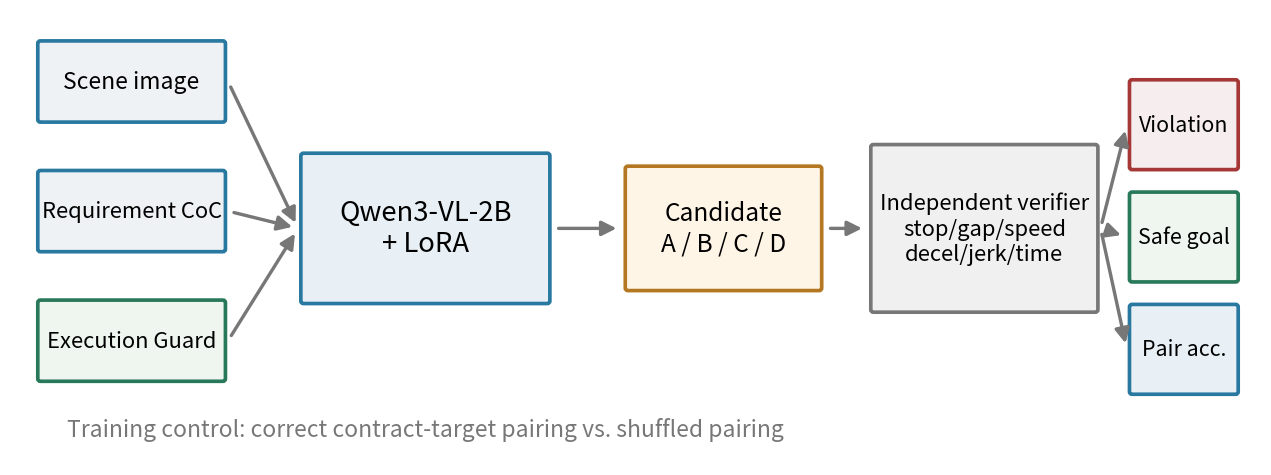
\includegraphics[width=0.98\textwidth]{figures/fig02_pipeline.png}
\caption{Safety-Constrained CoC의 입력, 궤적 후보 선택 및 독립 검증 과정. 모델은 후보 하나를 선택하고, 별도의 검증기가 선택된 후보의 목표 달성과 가드 준수를 판정한다.}
\label{fig:pipeline}
\end{figure*}

\subsection{CoC와 실행 가드의 입력 방식}

본 연구는 기본 CoC에 실행 가드를 결합한 형식을 제안한다. 예를 들어 기본 CoC가 "횡단보도 앞 보행자에게 양보한 뒤, 허용되면 진행한다"라면 다음 조건을 덧붙일 수 있다.

\begin{quote}\small
정지선을 넘지 않는다. 최대 감속도는 $3.8\,\mathrm{m/s^2}$, 최대 가가속도는 $5.0\,\mathrm{m/s^3}$를 넘지 않는다. 상충 구역이 정해진 시간 동안 비어 있을 때만 출발한다.
\end{quote}

이 실행 가드를 기본 CoC 뒤에 이어서 한 문장 묶음으로 제시한 방식을 \textbf{CoC 통합형}이라 한다. 모델은 이 입력에서 "무엇을 해야 하는가"와 "그 행동을 언제 허용하는가"를 함께 읽는다. 다만 성능이 좋아지더라도 그 이유가 가드의 의미를 배웠기 때문인지, 단순히 문장이 더 길어졌기 때문인지 구분해야 한다. 이를 위해 표~\ref{tab:representations}의 다섯 방식을 비교한다.

\begin{table*}[!t]
\centering
\caption{CoC와 실행 가드를 모델에 제시하는 다섯 가지 방식.}
\label{tab:representations}
\footnotesize
\begin{tabularx}{\textwidth}{L{0.19\textwidth}L{0.25\textwidth}Y}
\toprule
조건 & 모델에 주는 정보 & 비교 목적 \\
\midrule
요구사항 전용형 & 기본 CoC만 제시 & 실행 가드가 없을 때 장면과 행동 목표만으로 후보를 고르는 기준선 \\
CoC 통합형 & 기본 CoC 뒤에 실행 가드를 이어서 제시 & 요구사항과 실행 조건을 한 문맥에서 함께 학습하는 제안 조건 \\
가드 분리형 & 기본 CoC와 실행 가드를 서로 다른 항목으로 제시 & 같은 내용을 분리해서 제시했을 때의 차이 확인 \\
대응을 섞은 가드 & 가드 문장은 주지만 학습할 때 정답 후보와의 대응을 바꿈 & 문장이 추가된 효과와 올바른 가드 의미를 학습한 효과를 구분 \\
논리식 가드 & 실행 조건을 정해진 논리식으로 제시 & 자연어가 아닌 구조화된 표현을 현재 모델이 처리할 수 있는지 확인 \\
\bottomrule
\end{tabularx}
\end{table*}

특히 "대응을 섞은 가드"는 문장의 길이와 의미의 효과를 나누어 보기 위한 조건이다. 이 조건에도 가드 문장은 들어 있지만, 학습할 때 가드와 정답 후보를 일부러 잘못 연결한다. CoC 통합형은 잘 맞고 이 조건은 맞지 않는다면, 단순히 문장이 추가되어서가 아니라 올바른 가드-행동 관계를 배웠다고 해석할 수 있다. "논리식 가드"는 자연어 대신 정해진 기호 형식으로 같은 조건을 준다. 이 비교는 자연어와 논리식 중 어느 쪽이 본질적으로 우수한지 판정하려는 것이 아니라, 현재 VLM과 학습 방법이 두 표현을 얼마나 잘 처리하는지 확인하기 위한 것이다.

\subsection{같은 장면에서 실행 조건만 바꾸는 평가}

한 장면으로 정답이 서로 다른 두 문제를 만든다. 두 문제에는 같은 이미지, 같은 CoC 목표와 같은 궤적 후보를 사용한다. 바꾸는 것은 실행 가드뿐이다. 가드가 달라지면 올바른 후보도 달라지게 구성한다. 따라서 모델이 두 문제를 모두 맞히려면 장면만 보고 같은 답을 반복해서는 안 되고, 가드를 읽은 뒤 선택을 바꾸어야 한다. 이 두 문제의 묶음을 \textbf{쌍대 계약(paired-contract)}이라 한다.

그림~\ref{fig:pair}은 차선 변경 예에서 무엇이 고정되고 무엇이 바뀌는지를 보여준다. 두 계약 모두 현재 차량 간격은 7.2 m이며 후보도 같다. 후보 A는 현재 간격에서 바로 차선을 변경하고, 후보 B는 차선 변경을 중단한 뒤 필요한 간격이 확보되면 다시 시도한다. 최소 간격이 5.5 m인 완화 계약에서는 $7.2 \geq 5.5$이므로 후보 A가 허용되고 진행도가 높은 후보 A를 선택한다. 반면 최소 간격이 9.0 m인 엄격 계약에서는 $7.2 < 9.0$이므로 후보 A가 가드를 위반하고 후보 B를 선택해야 한다.

즉, 완화 계약과 엄격 계약은 장면이 아니라 허용 기준만 다르다. 모델이 두 문제에 같은 후보를 답하면 적어도 하나는 틀린다. "계약 전환 쌍 정확도"는 두 문제를 모두 맞혔을 때만 그 쌍을 정답으로 계산한다. 이 값이 높을수록 모델이 최소 간격의 변화를 읽고 선택에 반영했다고 볼 수 있다.

\begin{figure*}[!t]
\centering
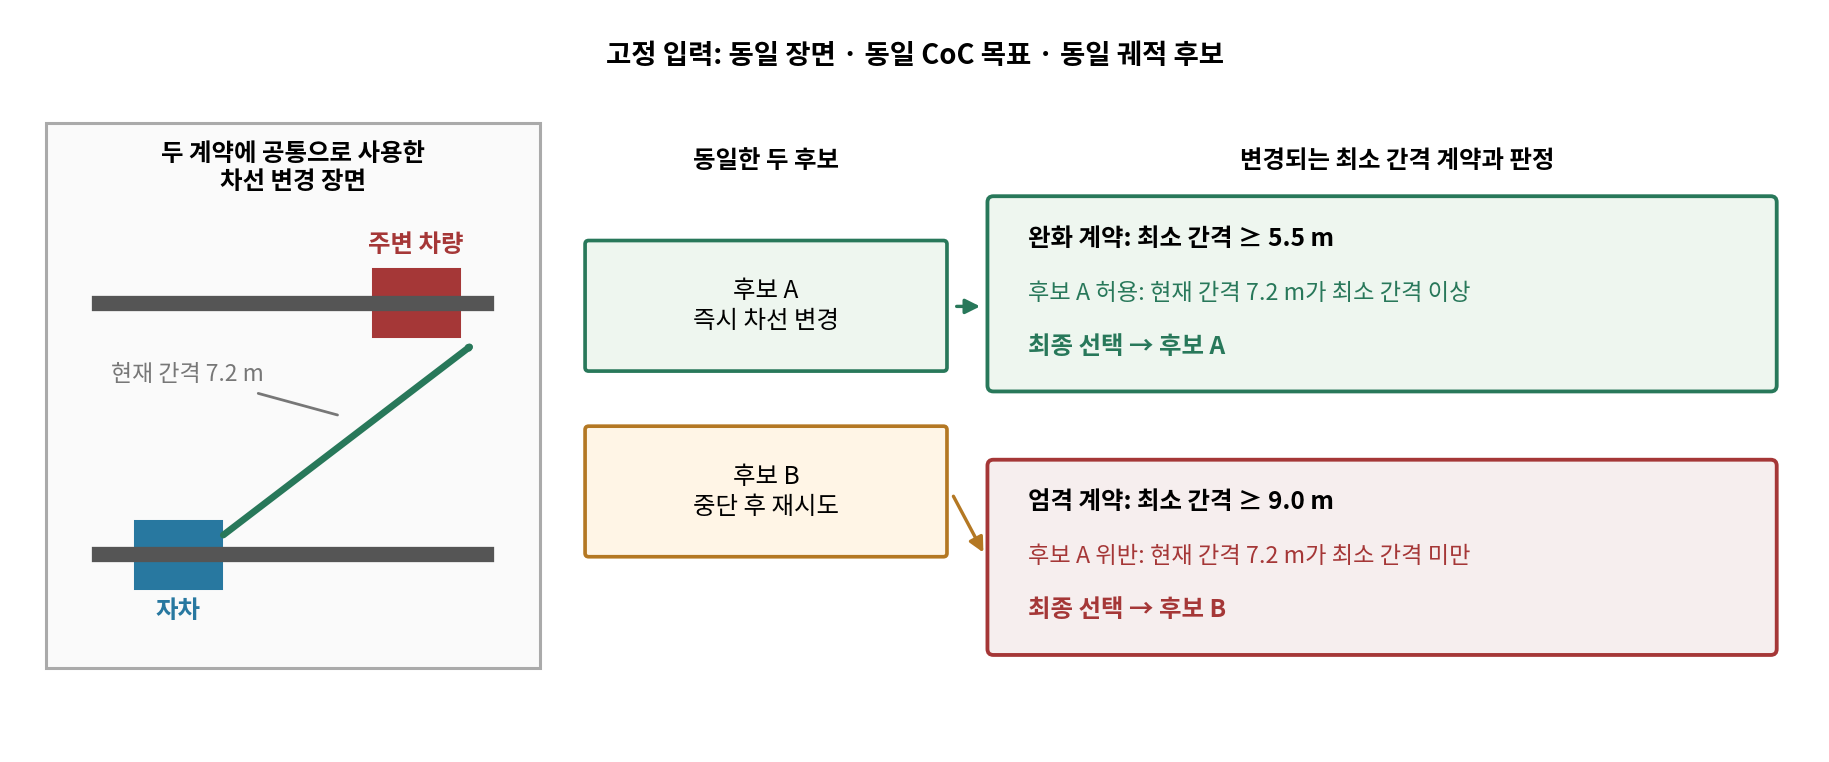
\includegraphics[width=0.98\textwidth]{figures/fig03_paired_contract.png}
\caption{쌍대 계약의 차선 변경 예. 장면, CoC 목표, 현재 간격 7.2 m 및 후보 A/B는 고정하고 최소 간격만 5.5 m에서 9.0 m로 바꾼다. 완화 계약에서는 즉시 차선 변경하는 후보 A가 허용되지만, 엄격 계약에서는 같은 후보가 최소 간격을 위반하므로 중단 후 재시도하는 후보 B를 선택한다.}
\label{fig:pair}
\end{figure*}

시간 과제에서는 행동이 다른 네 후보를 사용한다. 모델은 $A$, $B$, $C$, $D$ 중 하나를 답하지만, 이 문자는 후보를 구별하기 위한 이름일 뿐이다. 예를 들어 $A$가 언제나 조기 진입을 뜻하는 것은 아니다. 표~\ref{tab:candidate-roles}은 후보가 실제로 수행하는 네 가지 행동을 보여준다.

\begin{table*}[!t]
\centering
\caption{시간 과제의 네 궤적 역할과 계약에 따른 판정 예.}
\label{tab:candidate-roles}
\footnotesize
\begin{tabularx}{\textwidth}{L{0.18\textwidth}L{0.29\textwidth}L{0.20\textwidth}Y}
\toprule
궤적 역할 & 행동 & 완화 계약 & 엄격 계약 \\
\midrule
조기 진입 & 상충 구역이 비기 전에 진입 & 가드 위반 & 가드 위반 \\
짧은 대기 후 진입 & 상충 구역이 빈 뒤 짧게 기다리고 진행 & 선택 가능 & 대기시간 부족으로 위반 \\
긴 대기 후 진입 & 충분한 확인 시간을 거친 뒤 진행 & 허용되지만 진행이 느림 & 목표를 완료하는 적절한 후보 \\
계속 정지 & 평가 시간이 끝날 때까지 정지 & 목표 미완료 또는 교착 & 목표 미완료 또는 교착 \\
\bottomrule
\end{tabularx}
\end{table*}

한 장면에서는 $A$가 조기 진입이고 $B$가 짧은 대기일 수 있다. 다음 장면에서는 문자와 행동의 대응을 바꾸어 $A$가 긴 대기를 나타내게 할 수 있다. 이렇게 하면 모델이 항상 같은 문자만 고르는 방법으로 정답을 외울 수 없다. 정적 실험은 두 후보 $A/B$를, 시간 및 다중 주행 실험은 네 후보 $A/B/C/D$를 사용한다. 어느 실험에서도 특정 문자가 항상 안전하거나 항상 위험한 행동을 뜻하지 않는다.

\subsection{모델 학습과 정답 후보 생성}

기반 모델은 Qwen3-VL-2B-Instruct이다. 전체 모델을 다시 학습하지 않고 일부 추가 매개변수만 조정하는 LoRA 방식을 사용한다. 모델이 한 번에 받는 학습 자료는 다음 다섯 부분으로 구성된다.

\begin{enumerate}
\item 장면을 나타내는 합성 이미지,
\item 달성해야 할 행동을 설명하는 기본 CoC,
\item 실험 조건에 따른 실행 가드,
\item 각 후보의 행동과 측정값을 적은 설명,
\item 허용되는 후보 중 진행도가 가장 높은 후보를 고르라는 지시.
\end{enumerate}

모델은 후보 문자 하나를 답한다. 정답은 다음 세 단계로 정한다. 먼저 CoC의 행동 목표를 끝내지 못한 후보를 제외한다. 그다음 실행 가드를 위반한 후보를 제외한다. 마지막으로 남은 후보 중에서 가장 원활하게 진행하는 후보를 정답으로 삼는다. 모든 장면에는 목표와 가드를 함께 만족하는 후보가 적어도 하나 있다. 이는 식~\eqref{eq:selection}을 학습 자료 생성에 그대로 적용한 것이다.

예를 들어 가장 빨리 진행하는 후보가 최소 간격을 위반하면 정답이 될 수 없다. 반대로 가드 위반을 피하기 위해 끝까지 정지하는 후보도 행동 목표를 완료하지 못하므로 정답이 아니다. 모델은 "진행"과 "가드 준수"를 동시에 만족하는 후보를 찾아야 한다.

\subsection{독립 궤적 검증과 평가 지표}

모델의 답은 $A$와 같은 후보 문자일 뿐이다. 이 답이 실제로 가드를 지켰는지는 별도 검증기가 계산한다. 검증기는 표~\ref{tab:verifier-fields}의 수치를 후보 데이터에서 읽고 가드의 기준과 직접 비교한다. 예를 들어 최소 간격이 9.0 m라면 선택한 후보의 간격이 9.0 m 이상인지 확인한다.

\begin{table}[t]
\centering
\caption{독립 검증기가 확인하는 주요 값.}
\label{tab:verifier-fields}
\footnotesize
\begin{tabularx}{\columnwidth}{L{0.34\columnwidth}Y}
\toprule
확인 값 & 판정 예 \\
\midrule
정지선 기준 위치 & 0 m보다 크면 정지선을 넘어선 것으로 판정 \\
최대 속도 & 허용된 속도 상한을 넘는지 확인 \\
최대 감속도 & 급격한 감속 한계를 넘는지 확인 \\
최대 가가속도 & 가속도 변화가 허용 한계를 넘는지 확인 \\
최소 차량 간격 & 다른 차량과 필요한 거리를 유지하는지 확인 \\
교차로 진입 시점 & 상충 구역이 빈 뒤 필요한 대기시간을 지켰는지 확인 \\
\bottomrule
\end{tabularx}
\end{table}

표~\ref{tab:method-metrics}은 평가에 사용한 지표를 정리한다. 이 가운데 "가드 준수 목표 완료율"은 두 가지를 동시에 만족한 비율이다. 첫째, 선택한 후보가 CoC의 행동 목표를 완료해야 한다. 둘째, 실험에서 제시한 실행 가드를 모두 지켜야 한다. 이 지표는 실제 도로의 모든 위험이 제거되었다는 뜻은 아니다.

\begin{table}[t]
\centering
\caption{주요 평가 지표와 의미.}
\label{tab:method-metrics}
\footnotesize
\begin{tabularx}{\columnwidth}{L{0.31\columnwidth}Y}
\toprule
지표 & 의미 \\
\midrule
후보 정확도 & 모델이 데이터 생성 규칙으로 정한 최적 후보를 선택한 비율 \\
가드 위반률 & 선택한 후보가 하나 이상의 실행 가드를 위반한 비율 \\
가드 준수 목표 완료율 & 선택한 후보가 실행 가드를 지키면서 기본 CoC의 행동 목표도 완료한 비율 \\
교착률 & 가드를 위반하지 않지만 계속 정지하여 행동 목표를 완료하지 못한 비율 \\
과도한 보수 선택률 & 가드는 지키지만 같은 계약에서 허용되는 더 높은 진행도의 후보가 있는데도 지나치게 느린 후보를 고른 비율 \\
계약 전환 쌍 정확도 & 같은 장면의 완화 계약과 엄격 계약을 모두 맞힌 쌍의 비율 \\
\bottomrule
\end{tabularx}
\end{table}

일반 후보 정확도는 두 문제 중 하나만 맞혀도 각각의 정답으로 센다. 반면 계약 전환 쌍 정확도는 완화 계약과 엄격 계약을 모두 맞혀야 1로 센다. 따라서 이 지표는 모델이 가드가 바뀔 때 후보 선택도 바꾸었는지를 더 엄격하게 보여준다.

\subsection{학습된 가드 준수와 실제 실행 안전의 구분}

본 연구가 확인하는 것은 모델이 주어진 후보 중에서 가드를 지키는 후보를 더 잘 고를 수 있는가이다. 이것은 실제 차량에서 충돌을 막는 안전 보장과 다르다. 여기서 사용한 검증기는 실험 결과를 계산하는 도구이며, 차량의 명령을 실시간으로 막거나 수정하는 차단 장치가 아니다.

실제 차량에 적용하려면 두 단계가 더 필요하다. 먼저 자연어 가드에서 조건의 종류, 비교 방향, 수치, 단위와 조건을 지킬 수 없을 때의 대체 행동을 정확히 추출해야 한다. 예를 들어 "최소 간격 9 m"를 "거리, 이상, 9, m"처럼 일정한 형식으로 바꾸고 단위도 통일해야 한다. 다음으로 모델이 만든 궤적을 독립 검증기나 실행 차단 장치가 다시 검사해야 한다. 따라서 본 연구는 제한된 후보 선택 과제에서 가드 준수를 학습할 수 있음을 보일 뿐, 실제 도로의 완전한 안전 명세나 차량 안전을 보장하지 않는다.
